%\documentclass[12pt]{amsart}
\documentclass[12pt,notitlepage]{article}

\usepackage{geometry}                % See geometry.pdf to learn the layout options. There are lots.
\geometry{a4paper}                   % ... or a4paper or a5paper or ... 
%\geometry{landscape}                % Activate for for rotated page geometry
%\usepackage[parfill]{parskip}    % Activate to begin paragraphs with an empty line rather than an indent
\usepackage{graphicx}
\usepackage{amssymb}
\usepackage{epstopdf}
\usepackage{hyperref}
\usepackage{datetime}
%
\DeclareGraphicsRule{.tif}{png}{.png}{`convert #1 `dirname #1`/`basename #1 .tif`.png}

\title{Analysis of the San Francisco Crime Classification problem, from ``kaggle.com": a practical project in \emph{big data} and \emph{machine learning}}
\author{Stephen R. Williams}
\date{\today}  % Activate to display a given date or no date

\begin{document}
\maketitle

\begin{abstract}
This project is incomplete and ongoing. Here I explain the problem and document my efforts in competing in the \emph{kaggle} data science competition for \emph{San Francisco Crime Classification}. The problem aspires towards the optimal prediction for the likelihood for each of 39 possible crime categories having occurred, given a training data set and measured against the test data set. The data features can be divided into two broad categories, firstly the precise time and date at which the crime was reported to police (temporal features), and secondly the location where it occurred (spatial features). Here I will steadily and systematically build up towards my chosen approach. This approach will combine a variation on a \emph{naive Bayes} method with a \emph{random forest}. We will treat the temporal features as being independent of each other and of the spatial features, with the \emph{random forest} applied to the spatial features. In addition we predict the time dependent behaviour by exploiting the cyclic nature of human behaviour. The analysis will strongly exploit data feature engineering. \emph{Python} is the main software tool used throughout this project to implement the \emph{data science} (making use of both \emph{pandas} and \emph{sklearn} libraries), with \emph{R} to also be used.
\end{abstract}

The latest version of this document and all of the source files for the work it refers to are publicly available from my \emph{GitHub} repository, \url{https://github.com/wilstep/frisco-crime}

\section{Introduction (\emph{The Problem})}

The competition may be found at \url{https://www.kaggle.com/c/sf-crime} The problem consists of crime reports to the San Francisco police over the period 1/01/2003 through to 13/05/2015 with alternating weeks divided between the \emph{test data set} and the \emph{training data set}. The data set has the following data features (with some only in the training set (noted as: train.csv)),

\begin{itemize}
\item Dates - timestamp of the crime incident
\item Category - category of the crime incident (only in train.csv). This is the target variable you are going to predict.
\item Descript - detailed description of the crime incident (only in train.csv)
\item DayOfWeek - the day of the week
\item PdDistrict - name of the Police Department District
\item Resolution - how the crime incident was resolved (only in train.csv)
\item Address - the approximate street address of the crime incident 
\item X - Longitude
\item Y - Latitude,
\end{itemize}
%
and we are required to predict the \emph{Category} for the test set. The \emph{Category} provides which of the 39 possible crime categories has been recorded, e.g. Assault, Burglary, Fraud, etc.  There is not enough information available to predict the particular crime \emph{Category} with any reliability, and the aim is to predict the likelihood of each of the 39 possible category outcomes as best we can with the available information. This is forced upon us by the way our entries are scored, using a \emph{multi-class logarithmic loss} formula
%
\begin{equation}
logloss = -\frac{1}{N}\sum_{i=1}^N \sum_{j=1}^M y_{ij} \ln(p_{ij}),\label{eq:logloss}
\end{equation}
%
where $N=884,262$ is the number of crime incidents in the test set, $M=39$ is the number of possible crime category outcomes, $y_{ij}$ is unity if the 
actual (not known to us) crime category for incident $i$ happens to coincide with category $j$ and zero otherwise, $p_{ij}$ is the probability we have 
predicted for category $j$ being the actual (not known to us) crime category reported for crime incident $i$, and $\ln(x)$ is the natural logarithm of $x$. It is important to note that we do not have the required information available to compute the value of Eq. (\ref{eq:logloss}) for our results from the test data. This information is kept secret from us by the \emph{kaggle} administrators. However they do have the information and when an entry is submitted a score is reported back. A live leader board for these scores is maintained at \url{https://www.kaggle.com/c/sf-crime/leaderboard}

Given a suitable mathematical background, it is easy to see that this $logloss$ quantity has the property that the absolute statistical errors in our predictions for each of the 39 categories, contribute in proportion to their relative error. This means that it is important to put effort into accurately predicting the probability of not just the most likely outcomes, but also the not so likely outcomes. One should realise that if we correctly identify an outcome as being very unlikely, then as a result it's absolute error must be correspondingly very small, and that will be good enough. Let us start by making a submission that makes use of this observation, and very little more.

\section{Trial 1: An entropic approach}
Given Eq. (\ref{eq:logloss}) let us consider the optimal way of scoring upon ignoring all information based on time and space. That is, if we submit the same 39 probabilities for all of the $N=884,262$ crime incidents, what is the optimal probability weighting? In the limit where $N\rightarrow \infty$ this score will be given by the entropy
%
\begin{equation}
S = -\frac{1}{39}\sum_{j=1}^{39} p_j \ln{p_j},
\end{equation}
where $p_j$ is the global probability for the $j_{th}$ crime category occurring, and in this limit the global probabilities will correspond to the optimal probability weightings. I will not go into the details of how and why this is the case, and just hope that you accept my assertion of it being so. With this in mind let us compute the global probabilities for each of the 39 crime categories, using the training data, then compute the entropy, and see what happens upon making a \emph{kaggle} submission. But first lets see what these global probabilities look like.
%
\begin{figure}
\centering{}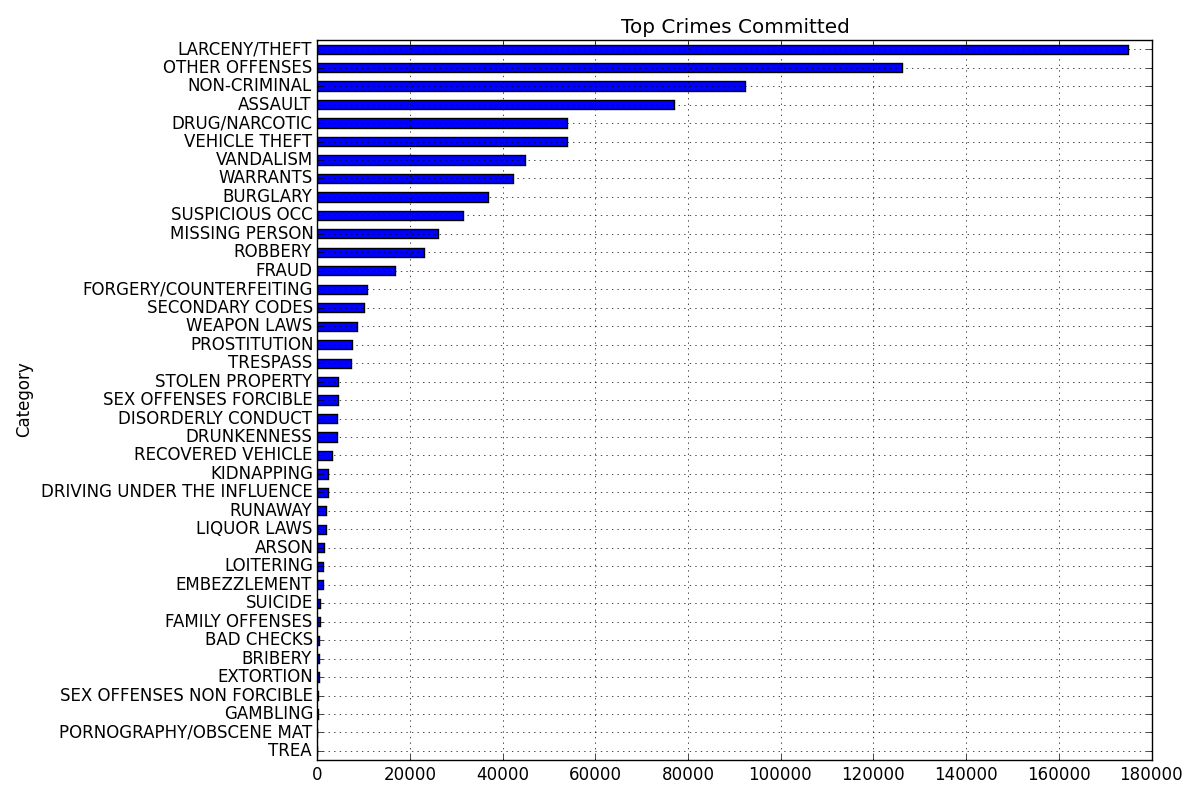
\includegraphics[scale=0.4]{crime-histo}\caption{ Histogram of crime categories, ranked from most to least prevalent. The $x$-axis gives the number of crime incidents over the full $12.4$ year period.  \label{fig:crime-hist}}
\end{figure}
%
There are some good graphing scripts that have been put up by the community on the \emph{kaggle} site. I have slightly modified one of these to make a histogram of the various crime categories ordered by their prevalence. The \emph{Python} script is here in my GitHub repository as ``entropy\textbackslash crime-graphs.py" and the relevant graph can be seen in Fig. (\ref{fig:crime-hist}). On average there are $884,262 / 39 \simeq 22,700$ crime reports per category (the frequency), and from the graph we see that the top crime category of LARCENY/THEFT is around 8 times more likely than the average, the twelfth most prevalent crime of ROBBERY is close to the average value, and by the time we are half way through the list of categories (say STOLEN PROPERTY) we are down to a frequency that is approximately 5 times less than the average. The top quarter to a third of most prominent categories contain the vast majority of all crime occurrences.  

Given our script for making the histogram, it is straightforward to also compute the entropy and output a submission file using the already computed
frequencies to obtain the global probabilities. I start a new script, ``entropy\textbackslash global-prob.py", which does this after initially printing out the
number of crime occurrences for each category (n.b. this script takes a little time to run). We see that the entropy has a value of $S = 2.68033$ and the
score given by the \emph{kaggle} entry is 2.68016, very similar indeed. This is a very unsophisticated entry; the competition started on the $2^{nd}$
June 2015 and when I submitted this on the $16^{th}$ of June it came in at position 52 out of 82 entries. At the time of writing $7^{th}$ July the best score is 2.27804. Given how rudimentary and crude this first entry is, it has done remarkably well.  

The reader might well ponder the importance of what has been done here. Consider how I have put forward a couple of assertions, and have shown how one of these is consistent with the outcome we obtained for our first submission, i.e. the score was extremely close to the value given by the entropy. These assertions (which can be mathematically proved) have lead me to the conclusion that we need to accurately predict not just the most probable outcomes, but also the less likely outcomes. While the outcome for our submission was overall not great, upon accounting for how simple and crude our method was, it was surprisingly effective. This shows the importance of having an approach that attempts to accurately predict all the possible outcomes, and thus it is crucial that we continue to heed this aspect as we move forward. 

\section{The Temporal problem addressed through sub-division}

To improve our method, we will make use of what time the crime occurred at. We will derive three different data features from the time stamp, making use of the the number of crimes that have occurred for each category, $N_c$, obtained from the training data. These derived data features are:  
\begin{itemize}
\item For each category, initially divide the $N_c$ data points into $m_c$ sub-divided blocks, representing equally spaced time segments. We make the integer $m_c$ as large as we can such that $m_c\leqslant16$, and that $(N_c + N_{min})/m_c \geqslant N_{min}$. If $N_c<N_{min}$ we don't make any subdivisions. This is done to handle slow drift in the data. We will denote this data feature as $d_{tdr}.$ We will end up setting  $N_{min}=1000$
\item The day of the week, changing at 6am, is used provided that $N_c\geqslant7000$. The 6am boundary is chosen because
criminal activity is at a low ebb at this time. We will denote this data feature as $d_{tdy}.$
\item The hour of the day, provided $N_c\geqslant24,000$. We will denote this data feature as $d_{thr}.$
\label{list-1}
\end{itemize}

To provide some insight for the motivation behind these choices we will first consider some highly relevant graphs. We know that humans tend to organise their lives around the clock and the calendar. For this reason various crimes may be more prevalent at certain times or days of the week, and also depend upon the season. For example wallets may be more likely to be stolen from the beach during the day time in the summer, etc. Initially I attempted to analyse this periodicity through a Fourier analysis, but that proved ineffective. However I leave the Fourier predictions in the graphs I present here, as it does no harm. We will focus on the typical time scales on which humans organise their behaviour and home in on the time scales that are important. Fortunately this is rather straightforward using the training data. 

\begin{figure}
\centering{}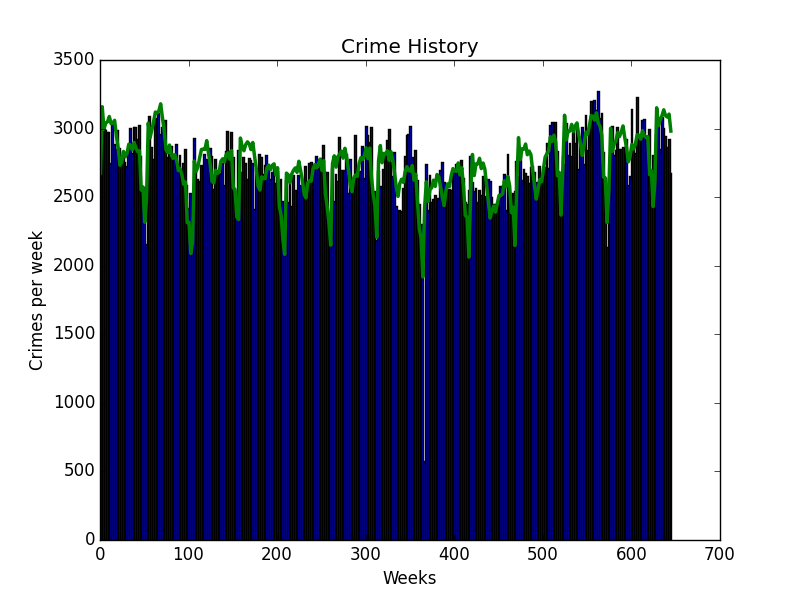
\includegraphics[scale=0.7]{time-1}\caption{ Histogram of crimes per week (all crime categories combined) and Fourier series (solid green line) estimate of the same, over the entire time period of 12.4 years spanned by the training data.\label{fig:time-1}}
\end{figure}
%
The first graph we consider shows a histogram of the sum of all the crime categories over the full 12.4 years (645 weeks) spanned by the data. The Python script ``Fourier\textbackslash time-1.py", which makes use of ``Fourier\textbackslash fourier.py", produces this histogram, Fig. (\ref{fig:time-1}). We can see how the crime rate fluctuates and drifts. Given the long time period that this data spans, the drift is to be expected. When we consider specific crime categories we can expect these behaviours to become more pronounced, as a result of the law of large numbers. We now focus on a much shorter time scale for the exact same data, Fig (\ref{fig:time-2}), see ``Fourier\textbackslash time-2.py". Here we see how the crime rate is strongly dependent on the time of the day and to a lesser extent the day of the week. The crime rate slows right down in the early morning and is less active on a Sunday.
%
\begin{figure}
\centering{}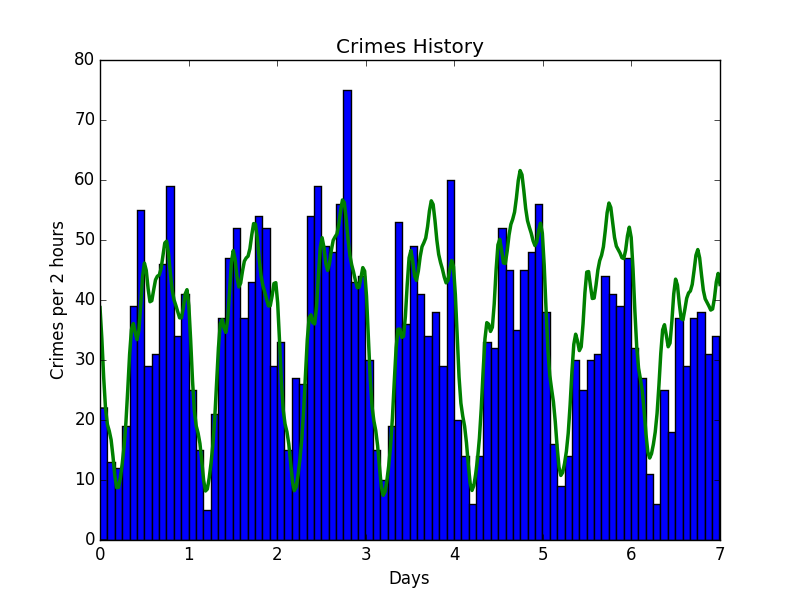
\includegraphics[scale=0.7]{time-2}\caption{ Histogram of crimes per 2 hour period over the first week of training data and Fourier series 
(solid green line) estimate of the same, over the first week spanned by the training data. The data for \emph{Days} starts at 00:00 hours Monday\label{fig:time-2}}
\end{figure}
%
Let us now take a look at some graphs of specific crime categories. In Fig. (\ref{fig:time-3}) we plot a histogram for the category of \emph{Vehicle Theft} over the full 12.4 years spanned by the data. The script to compute this is given in ``Fourier\textbackslash time-3.py". Here we see that the drift is far more dramatic than was the case for the sum of all the categories in Fig. (\ref{fig:time-1}). Importantly there is an artefact in this data seen as a sudden drop in the rate of thefts around the 150 week mark. The reason for this is not of primary concern to us, just so long as our approach makes use of this information. Referring back to the first point in our list of derived data features at the start of this section, we see that the first derived data feature is just what we need to handle this type of artefact. 

We will now construct another two graphs along similar lines to Fig. (\ref{fig:time-2}), but for specific crime categories. We will look at two categories of particular interest, firstly \emph{Larceny/Theft} because it is the most prevalent as can be seen in Fig. (\ref{fig:crime-hist}) and secondly \emph{Drunkenness}. One would expect \emph{Drunkenness} may be interesting from a temporal perspective because people tend to get in trouble for it on the weekend and at night. So this is a crime that may stand out as happening at atypical times.
%
\begin{figure}
\centering{}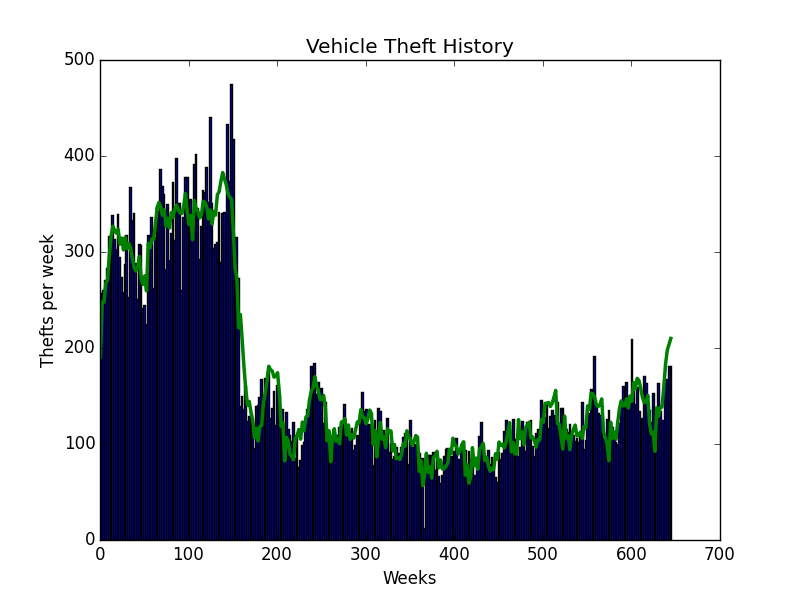
\includegraphics[scale=0.7]{time-3}\caption{ Histogram of vehicle thefts per week and Fourier series (solid green line) estimate of the same, over the entire time period of 12.4 years spanned by the training data.\label{fig:time-3}}
\end{figure}
%\begin{figure}
%\centering{}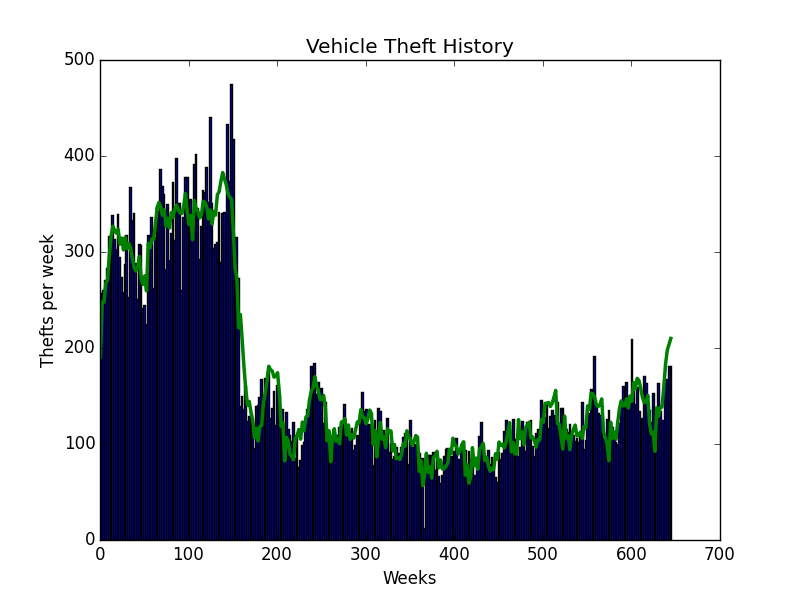
\includegraphics[scale=0.7]{time-3}\caption{ Histogram of Larceny/Theft per two hours, accumulated over the first 100 weeks of the test data 
%and Fourier series (solid green line) estimate of same. The data for \emph{Days} starts at 00:00 hours Monday\label{fig:time-3}}
%\end{figure}
%
The graph for \emph{Larceny/Theft} crime category is shown in Fig. (\ref{fig:time-4}) and was made using the script `Fourier\textbackslash time-4.py". We have summed up the training data (we only have every second week) over a duration of 100 weeks here. We can see that much like was the case for the sum of all the categories shown in Fig. (\ref{fig:time-2}) the rate for this crime category tends to be pretty low early in the morning, around 06:00. 

We now move onto the Drunkenness category. 
%
\begin{figure}
\centering{}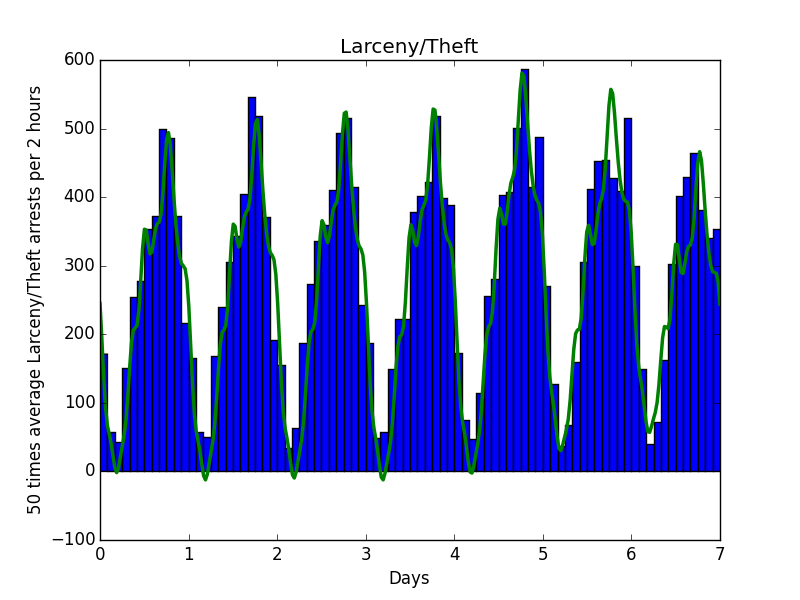
\includegraphics[scale=0.7]{time-4}\caption{ Histogram of Larceny/Theft per two hours, accumulated over the first 100 weeks of the test data 
and Fourier series (solid green line) estimate of same. The data for \emph{Days} starts at 00:00 hours Monday\label{fig:time-4}}
\end{figure}
%
%
\begin{figure}
\centering{}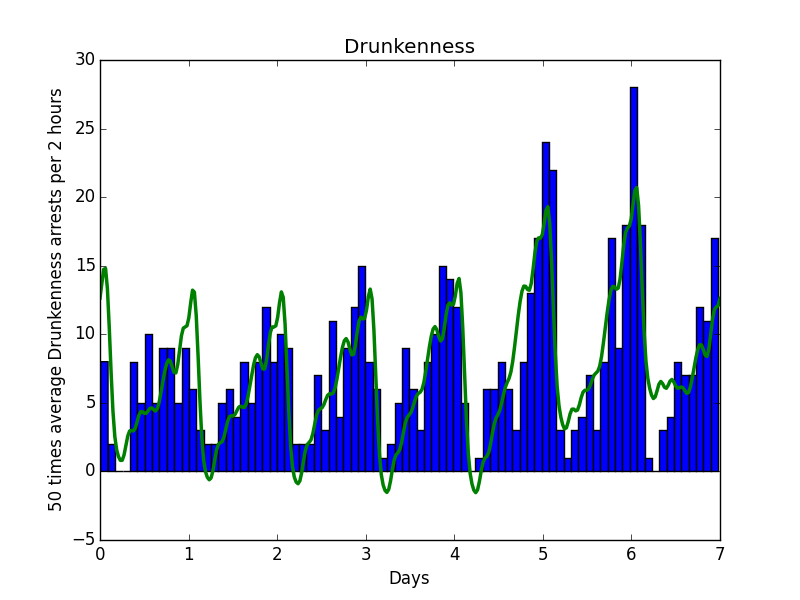
\includegraphics[scale=0.7]{time-5}\caption{ Histogram of \emph{Drunkness} per two hours, accumulated over the first 100 weeks of the test 
data and Fourier series (solid green line) estimate of same. The data for \emph{Days} starts at 00:00 hours Monday\label{fig:time-5}}
\end{figure}
%
The graph for the \emph{Drunkenness} crime category is shown in Fig. (\ref{fig:time-5}) and was made using the script ``Fourier\textbackslash time-5.py". Here we see some interesting behaviour that is quite different to what we saw in the sum of all the categories shown in Fig. (\ref{fig:time-2}). There are notably more cases of \emph{Drunkenness} on Friday and Saturday night, and the data is skewed towards late in the evening. 

So let's now see what we can do to implement this data, using the the derived data features that we have listed at the top of this section. We implement this in the script, ``time-sub-div\textbackslash sdiv.py". Upon  assuming each of our features to be independent we can express the probability in terms of our temporal features as
%
\begin{equation}
P(f_{cr}|{\bf d_t})  \propto P(f_{cr}) \frac{P(f_{cr}|d_{tdr})P(f_{cr}|d_{tdy})P(f_{cr}|d_{thr})}{P^3(f_{cr})},
\end{equation}
where ${\bf d_t} = [d_{tdr},d_{tdy},d_{thr}]$ is a vector representing all the temporal features, $f_{cr}$  is the crime category and $P(f|x)$ is the conditional probability of observing $f$ given we have the value $x$. This is very similar to what is done in a Bernoulli naive Bayes classifier, except we compute the posterior directly rather than obtaining it from the prior. This is convenient here as it will make it easier to experiment with feature engineering and adding a random forest as we progress further.
	So we implement this simple approach in the Python script ``time-sub-div\textbackslash sub.py", which has several parameters that may be altered. First we implement this using only the drift variable which has the parameter $N_{min}$ as given in the list at the beginning of this section. I settled on a value of $N_{min} = 1000$ that returned a score of 2.66062 which is an improvement on our earlier score of 2.68016. Next the day of the week, $d_{tdy}$, was additionally included with the parameter $D_{min}=2000$. This parameter represents the minimum number of crimes a given category must have recorded against it, if this data feature is to be used. This reduced the score further to 2.65794. Finally we additionally include the $d_{thr}$ feature, with the parameter $H_{min}$ which represents the minimum category score for the hour, just as was done for the day. This reduced the score further to 2.62751 which is our best improvement so far. 
	Thus far we have done enough to get about half way up the leaderboard (things become more competitive as time progresses). As it turns out the temporal features just aren't as strongly correlated with the crime categories as the spatial features are. However as we move further towards the top of the leaderboard, small improvements become more and more important. We will next move onto the spatial features and drop the temporal features for now. In the long run it will become important to combine both types of features.

\section{Using the spatial information}

There is quite a bit of information provided in the data features about the location where the crime occurred. Let us start by noting the police department (PD) that handled the crime. There are 10 separate PDs given, each of which has recorded a comparable number of the crimes over the 12.4 year duration. So let us start by making a simple submission based on the which PD the crime was handled by. To do this we simply enumerate the probability for each crime given the PD using the training data, and then use this with the PD provided for each crime in the test data. This is done by our script ``position\textbackslash sub-1.py" and resulted in a score of 2.61645 which is our best so far. So we see that the spatial features appears to have much stronger correlation than the temporal features. This is good because there is still much more we can do with the spatial features.

Let us now consider the address where the crime occurred. One of the interesting aspects about the address is that there are a small subset of addresses that have a disproportionately large number of crimes listed against them. Our script ``position\textbackslash worst-address.py" provides some basic statistics that bring this out very simply. There are 878,049 crimes provided in the training data and on average there are 37.8 crimes per address. Of these there are 83 addresses that have 750 crimes or more each against them. These 83 addresses account for 16.8\% of all crimes but only consist of 0.36\% of all addresses. This is good news for us, because this is something we can exploit. The precise address is very detailed information but a small subset of them are associated with a remarkably large portion of crime. So we can get good statistics on this small subset of addresses, and given the address is such specific information we should get very strong variability between the addresses. We will incorporate this into our script, by first determining if our crime happened at one of these addresses. If it did we will use the probabilities computed for the specific address, and if it didn't we will use the probabilities computed for the PD as we did previously. This is done in the script ``position\textbackslash sub-2.py" and this script now has a parameter we can vary called $Amin$ which is the minimum number of crimes an address must have if we are going to use it. We set $Amin = 1000$ and obtain the score 2.585. This has improved our position on the leader board considerably, to approximately two thirds the way to the top. But we still have quite a large amount of work to do and the strong exception that our position can be improved substantially.

\section{Moving forward}

For now we conclude this document by outlining the current plan moving forward. There is an important data feature we have yet to make use of. That is the GPS coordinate (X, Y) for where the crime occurred. In some cases these coordinates have an absurd value, presumably representative of a null recording, but these cases are firmly in the minority. We will make a 2 dimensional grid which covers San Fransisco. This grid will be composed of squares, all of the same size, and will have a parameter that determines the size (or equivalently the number) of the squares. We will arrange things such that the squares on average contain more crimes than the addresses do on average, but less than the PDs do on average. Then we will introduce an additional parameter $Gmin$, and arrive at the following; if the address has more than Amin crimes associated with it we will use the spatial statistics associated with that address, else if the grid position has more than $Gmin$ crimes associated with it we will use the statistics associated with that grid position, else failing either of these we will use the statistics associated with the PD. This approach of deciding which spatial feature to use depending upon the number of crimes associated with the various features is a form of \emph{feature engineering}. 

Having done this we can extend things further by retaining the important elements of the feature engineering, and then introducing a random forest method. Our previous hard work will be very useful for this, as we have systematically parameterised our feature engineering towards an optimal result, and we will be able to make good use of the code in our existing scripts. Finally we can bring the temporal features back to form an approach which makes good use of all of the data features. There is still plenty of scope for improvement before settling on our final result.

%$Amin = 1500$ score 2.59256 moved up 28 places, 26 addresses at or over 1500
%$Amin = 1000$ score 2.585 moved up a further 9 places, 50 addresses at or over 1000

%\section{}
%\subsection{}

\end{document}  